% ===== handout mode =====
% Comment/uncomment this line to toggle handout mode
% \newcommand{\handout}{}

% Comment/uncoment this line to toogle Mortitz mode
% \newcommand{\Moritz}{}

% Comment/uncomment this line to toggle handout mode
% \newcommand{\handout}{}

% by Stephan

%% Moritz mode or Stephan mode
\ifdefined \MoritzMode

% This is a configuration file with private, tutor specific information.
% It is therefore excluded from the Git repository so changes in this file will not conflict in git commits.

% Copy this Template, rename to config.tex and add your information below.

\newcommand{\mymail}{moritz.laupichler@student.kit.edu} % Consider using your named student Mail address to keep your u-Account private.

\newcommand{\myname}{\href{mailto:\mymail}{Moritz Laupichler}}

\newcommand{\mytutnumber}{27}

\newcommand{\mytutinfos}{Dienstags, 5. Block (15:45-17:15), SR 236}

\newcommand{\aboutMeFrame}{
	\begin{frame}{Euer Tutor}
		Name: \myname \\
		Alter: 19 Jahre \\
		Studiengang: Bachelor Informatik, 3. Semester \\
		\vspace{1cm}
		\pause 
		\centering{Kontakt: \href{mailto:\mymail}{\mymail}}
	\end{frame}
}

% Toggle Handout mode by including the following line before including style_tut
% and removing the % at the start (but do NOT remove it here, otherwise handout mode will always be on!)
% Please keep handout mode on in all commits!

% \newcommand{\handout}{} % Moritz mode
\fi
\ifdefined \AlexMode

% This is a configuration file with private, tutor specific information.
% It is therefore excluded from the Git repository so changes in this file will not conflict in git commits.

% Copy this Template, rename to config.tex and add your information below.

\newcommand{\mymail}{alexander.klug@student.kit.edu} % Consider using your named student Mail address to keep your u-Account private.

\newcommand{\myname}{\href{mailto:\mymail}{Alexander Klug}}

\newcommand{\mytutnumber}{30}

\newcommand{\mytutinfos}{Mittwochs, 3. Block (11:30-13:00), SR -107}

\newcommand{\aboutMeFrame}{
	\begin{frame}{Euer Tutor}
		Name: \myname \\
		Alter: 19 Jahre \\
		Studiengang: Bachelor Informatik, 3. Semester \\
		\vspace{1cm}
		\pause 
		\centering{Kontakt: \href{mailto:\mymail}{\mymail}}
	\end{frame}
}

% Toggle Handout mode by including the following line before including style_tut
% and removing the % at the start (but do NOT remove it here, otherwise handout mode will always be on!)
% Please keep handout mode on in all commits!

% \newcommand{\handout}{} % Alex Mode
\fi
\ifdefined \StephanMode

% This is a configuration file with private, tutor specific information.
% It is therefore excluded from the Git repository so changes in this file will not conflict in git commits.

% Copy this Template, rename to config.tex and add your information below.

\newcommand{\mymail}{stephan.bohr@student.kit.edu} % Consider using your named student Mail address to keep your u-Account private.

\newcommand{\myname}{\href{mailto:\mymail}{Stephan Bohr}}

\newcommand{\mytutnumber}{19}

\newcommand{\mytutinfos}{Dienstags, 3. Block (11:30-13:00), SR -108}

\newcommand{\aboutMeFrame}{
	\begin{frame}{Euer Tutor}
		Name: \myname \\
		Alter: 21 Jahre \\
		Studiengang: Bachelor Informatik, 5. Semester \\
		\vspace{1cm}
		\pause 
		\centering{Kontakt: \href{mailto:\mymail}{\mymail}}
	\end{frame}
} % Stephan mode
\fi

%% Beamer-Klasse im korrekten Modus
\ifdefined \handout
\documentclass[handout]{beamer} % Handout mode
\else
\documentclass{beamer}
\fi
%\documentclass[18pt,parskip]{beamer}

%% SLIDE FORMAT

% use 'beamerthemekit' for standard 4:3 ratio
% for widescreen slides (16:9), use 'beamerthemekitwide'

\usepackage{../templates/KIT-slides/beamerthemekit}
%\usepackage{../templates/KIT-slides/beamerthemekitwide}

%% TITLE PICTURE

% if a custom picture is to be used on the title page, copy it into the 'logos'
% directory, in the line below, replace 'mypicture' with the 
% filename (without extension) and uncomment the following line
% (picture proportions: 63 : 20 for standard, 169 : 40 for wide
% *.eps format if you use latex+dvips+ps2pdf, 
% *.jpg/*.png/*.pdf if you use pdflatex)

\titleimage{../figures/titleimage/brain}

%% TITLE LOGO

% for a custom logo on the front page, copy your file into the 'logos'
% directory, insert the filename in the line below and uncomment it

%\titlelogo{mylogo}

% (*.eps format if you use latex+dvips+ps2pdf,
% *.jpg/*.png/*.pdf if you use pdflatex)

%% TikZ INTEGRATION

% use these packages for PCM symbols and UML classes
% \usepackage{templates/tikzkit}
% \usepackage{templates/tikzuml}

%\usepackage{tikz}
%\usetikzlibrary{matrix}
%\usetikzlibrary{arrows.meta}
%\usetikzlibrary{automata}
%\usetikzlibrary{tikzmark}

%%%%%%%%%%%%%%%%%%%%%%%%%
% Libertine font (Original GBI font)
\usepackage[mono=false]{libertine}
%\renewcommand*\familydefault{\sfdefault}  %% Only if the base font of the document is to be sans serif

%% Schönere Schriften
\usepackage[TS1,T1]{fontenc}

%% Deutsche Silbentrennung und Beschriftungen
\usepackage[ngerman]{babel}

%% UTF-8-Encoding
\usepackage[utf8]{inputenc}

%% Bibliotheken für viele mathematische Symbole
\usepackage{amsmath, amsfonts, amssymb}

%% Anzeigetiefe für Inhaltsverzeichnis: 1 Stufe
\setcounter{tocdepth}{1}

%% Hyperlinks
\usepackage{hyperref}
% I don't know why, but this works and only includes sections and NOT subsections in the pdf-bookmarks.
\hypersetup{bookmarksdepth=subsection}

%% remove navigation symbols
\setbeamertemplate{navigation symbols}{}

%% switch between "ngerman" and "english" for German/English style date and logos
\selectlanguage{ngerman}

%% for invisible pause texts instead of dimming
\setbeamercovered{invisible}

\usepackage[german=swiss]{csquotes}

\usepackage{tabularx}
\usepackage{booktabs}

\usepackage{tikz}


% Problem: disabled itemize-icons
%\usepackage{enumitem}
% %\setlist[enumerate]{topsep=0pt,itemsep=-1ex,partopsep=1ex,parsep=1ex}
% \setlist[itemize]{noitemsep, nolistsep}
% \setlist[enumerate]{noitemsep, nolistsep}

% Mathmode no vertical space (https://tex.stackexchange.com/a/47403/146825)
\setlength{\abovedisplayskip}{0pt}
\setlength{\belowdisplayskip}{0pt}
\setlength{\abovedisplayshortskip}{0pt}
\setlength{\belowdisplayshortskip}{0pt}

%%%%%%%%%%%% Slides %%%%%%%%%%%%%%%%

\newcommand{\Moritz}[1]{
	\ifdefined \MoritzMode
	#1
	\fi
}

\newcommand{\Alex}[1]{
	\ifdefined \AlexMode
	#1
	\fi
}

\newcommand{\Stephan}[1]{
	\ifdefined \StephanMode
	#1
	\fi
}

\newcommand{\notMoritz}[1]{
	\Alex{#1} \Stephan{#1}
}

\newcommand{\notAlex}[1]{
	\Moritz{#1} \Stephan{#1}
}

\newcommand{\notStephan}[1]{
	\Alex{#1} \Moritz{#1}
}

%% Wochennummer
%\newcounter{weeknum}

%% Titelinformationen
%\title[GBI Tutorium, Woche \theweeknum]{Grundbegriffe der Informatik \\ Tutorium \mytutnumber}
%\subtitle{Termin \theweeknum \ | \mydate \\ \myname}
\author[\myname]{\myname}
\institute{Fakultät für Informatik}
%\date{\mydate}

%% Titel einfügen
\newcommand{\titleframe}{\frame{\titlepage}\addtocounter{framenumber}{-1}}


%% Alles starten mit \starttut{X}
%\newcommand{\starttut}[1]{\setcounter{weeknum}{#1}\titleframe\frame{\frametitle{Inhalt}\tableofcontents} \AtBeginSection[]{%
%\begin{frame}
%	\tableofcontents[currentsection]
%\end{frame}\addtocounter{framenumber}{-1}}}


%\newcommand{\framePrevEpisode}{
%	\begin{frame}
%		\centering
%		\textbf{In the previous episode of GBI...}
%	\end{frame}
%}

%% Roadmap frame
%table of contents
\newcommand{\roadmap}{
	\frame{\frametitle{Roadmap}\tableofcontents}}

 \AtBeginSection[]{%
\begin{frame}
	\frametitle{Roadmap}
	\tableofcontents[currentsection]
\end{frame}%\addtocounter{framenumber}{-1}
}


%% ShowMessage frame
\newcommand{\showmessage}[1]{\frame{\frametitle{\phantom{1em}}\centering\textbf{#1}}}

%% Fragen
%% Lastframe
\newcommand{\questionframe}{\showmessage{Fragen?}}

%% Lastframe
\newcommand{\lastframe}{\showmessage{Vielen Dank für Eure Aufmerksamkeit! \\Bis nächste Woche :)}}

%% Thanks frame
\newcommand{\slideThanks}{
	\begin{frame}
		\frametitle{Credits}
		\begin{block}{}
			An der Erstellung des Foliensatzes haben mitgewirkt:\\[1em]
			\Moritz{
			Stephan Bohr \\
			Alexander Klug \\
			}
			\Alex{
			Stephan Bohr \\
			Moritz Laupichler \\
			}
			\Stephan{
			Moritz Laupichler \\
			Alexander Klug \\
			}
			Katharina Wurz \\
			Thassilo Helmold \\
			Daniel Jungkind \\
			% Philipp Basler \\
			% Nils Braun \\
			% Dominik Doerner \\
			% Ou Yue \\
		\end{block}
	\end{frame}
}

%% Verbatim
%\usepackage{moreverb}

% GBI related stuff, but not beamer-stuff
\newcommand{\newpar}[1]{\paragraph{#1}\mbox{}\newline}

\newcommand{\nM}{\mathbb{M}}
\newcommand{\nR}{\mathbb{R}}
\newcommand{\nN}{\mathbb{N}}
\newcommand{\nZ}{\mathbb{Z}}
\newcommand{\nQ}{\mathbb{Q}}
\newcommand{\nB}{\mathbb{B}}
\newcommand{\nC}{\mathbb{C}}
\newcommand{\nK}{\mathbb{K}}
\newcommand{\nF}{\mathbb{F}}
\newcommand{\nG}{\mathbb{G}}
\newcommand{\nullel}{\mathcal{O}}
\newcommand{\einsel}{\mathds{1}}
\newcommand{\nP}{\mathbb{P}}
\newcommand{\Pot}{\mathcal{P}}
\renewcommand{\O}{\text{O}}

\newcommand{\bfmod}{\ensuremath{\text{\textbf{ mod }}}}
\renewcommand{\mod}{\bfmod}
\newcommand{\bfdiv}{\ensuremath{\text{\textbf{ div }}}}
\renewcommand{\div}{\bfdiv}


\newcommand{\set}[1]{\left\{ #1 \right\}}
\newcommand{\setc}[2]{\set{#1 \mid #2}}
\newcommand{\setC}[2]{\set{#1 \mid \text{ #2 }}}

\newcommand{\setsize}[1]{\; \mid #1 \mid \; }

\newcommand{\q}[1]{\textquotedblleft #1\textquotedblright}

% Zu zeigen, thx to http://www.matheboard.de/archive/155832/thread.html
\newcommand{\zz}{\ensuremath{\mathrm{z\kern-.29em\raise-0.44ex\hbox{z}}}:}

% Text above symbol
% https://tex.stackexchange.com/a/74132/146825
%
% \newcommand{\eqtext}[1]{\stackrel{\mathclap{\normalfont\mbox{#1}}}{=}}
% \newcommand{\gdwtext}[1]{\stackrel{\mathclap{\normalfont\mbox{#1}}}{\Leftrightarrow}}
% \newcommand{\imptext}[1]{\stackrel{\mathclap{\normalfont\mbox{#1}}}{\Rightarrow}}
% \newcommand{\symbtext}[2]{\stackrel{\mathclap{\normalfont\mbox{#2}}}{#1}}
\newcommand{\eqtext}[1]{\mathrel{\overset{\makebox%[0pt]
{\mbox{\normalfont\tiny #1}}}{=}}}
\newcommand{\gdwtext}[1]{\mathrel{\overset{\makebox%[0pt]
{\mbox{\normalfont\tiny #1}}}{\ensuremath{\Leftrightarrow}}}}
\newcommand{\imptext}[1]{\mathrel{\overset{\makebox%[0pt]
{\mbox{\normalfont\tiny #1}}}{\ensuremath{\Rightarrow}}}}
\newcommand{\symbtext}[2]{\mathrel{\overset{\makebox%[0pt]
{\mbox{\normalfont\tiny #2}}}{#1}}}

% qed symbol
\newcommand{\qedblack}{\hfill \ensuremath{\blacksquare}}
\newcommand{\qedwhite}{\hfill \ensuremath{\Box}}

% Aussagenlogik
% Worsch
\colorlet{alcolor}{blue}
\RequirePackage{tikz}
\usetikzlibrary{arrows.meta}
\newcommand{\alimpl}{\mathrel{\tikz[x={(0.1ex,0ex)},y={(0ex,0.1ex)},>={Classical TikZ Rightarrow[]}]{\draw[alcolor,->,line width=0.7pt,line cap=round] (0,0) -- (15,0);\path (0,-6);}}}
\newcommand{\alimp}{\alimpl}
\newcommand{\aleqv}{\mathrel{\tikz[x={(0.1ex,0ex)},y={(0ex,0.1ex)},>={Classical TikZ Rightarrow[]}]{\draw[alcolor,<->,line width=0.7pt,line cap=round] (0,0) -- (18,0);\path (0,-6);}}}
\newcommand{\aland}{\mathbin{\raisebox{-0.6pt}{\rotatebox{90}{\texttt{\color{alcolor}\char62}}}}}
\newcommand{\alor}{\mathbin{\raisebox{-0.8pt}{\rotatebox{90}{\texttt{\color{alcolor}\char60}}}}}
%\newcommand{\ali}[1]{_{\mathtt{\color{alcolor}#1}}}
\newcommand{\alv}[1]{\mathtt{\color{alcolor}#1}}
\newcommand{\alnot}{\mathop{\tikz[x={(0.1ex,0ex)},y={(0ex,0.1ex)}]{\draw[alcolor,line width=0.7pt,line cap=round,line join=round] (0,0) -- (10,0) -- (10,-4);\path (0,-8) ;}}}
\newcommand{\alP}{\alv{P}} %ali{#1}}
%\newcommand{\alka}{\negthinspace\hbox{\texttt{\color{alcolor}(}}}
\newcommand{\alka}{\negthinspace\text{\texttt{\color{alcolor}(}}}
%\newcommand{\alkz}{\texttt{\color{alcolor})}}\negthinspace}
\newcommand{\alkz}{\text{\texttt{\color{alcolor})}}\negthinspace}

% Thassilo
\newcommand{\BB}{\mathbb{B}}
\newcommand{\boder}{\alor}%{\ensuremath{\text{\;}\textcolor{blue}{\vee}}\text{\;}}
\newcommand{\bund}{\aland}%{\ensuremath{\text{\;}\textcolor{blue}{\wedge}}\text{\;}}
\newcommand{\bimp}{\alimp}%{\ensuremath{\text{\;}\textcolor{blue}{\to}}\text{\;}}
\newcommand{\bnot}{\alnot}%{\ensuremath{\text{\;}\textcolor{blue}{\neg}}\text{}}
\newcommand{\bgdw}{\aleqv}%{\ensuremath{\text{\;}\textcolor{blue}{\leftrightarrow}}\text{\;}}
\newcommand{\bone}{\ensuremath{\textcolor{blue}{1}}\text{}}
\newcommand{\bzero}{\ensuremath{\textcolor{blue}{0}}\text{}}
\newcommand{\bleftBr}{\alka}%{\ensuremath{\textcolor{blue}{(}}\text{}}
\newcommand{\brightBr}{\alkz}%{\ensuremath{\textcolor{blue}{)}}\text{}}

\newcommand{\val}{\hbox{\textit{val}}}

\newcommand{\VarAL}{\hbox{\textit{Var}}_{AL}}
\newcommand{\ForAL}{\hbox{\textit{For}}_{AL}}

% Validierungsfunktion val_i
\newcommand{\vali}[1]{\ensuremath{\val_I(#1)}}

% Boolsche Funktion b_
\newcommand{\bfnot}[1]{\ensuremath{b_{\bnot}(#1)}}
\newcommand{\bfand}[2]{\ensuremath{b_{\bund}(#1,#2)}}
\newcommand{\bfor}[2]{\ensuremath{b_{\boder}(#1,#2)}}
\newcommand{\bfimp}[2]{\ensuremath{b_{\bimp}(#1,#2)}}

% Aussagenkalkül
\newcommand{\AAL}{A_{AL}}
\newcommand{\LAL}{\hbox{\textit{For}}_{AL}}
\newcommand{\AxAL}{\hbox{\textit{Ax}}_{AL}}
\newcommand{\MP}{\hbox{\textit{MP}}}

% Prädikatenlogik
% die nachfolgenden Sachen angepasst an cmtt
\newlength{\ttquantwd}
\setlength{\ttquantwd}{1ex}
\newlength{\ttquantht}
\setlength{\ttquantht}{6.75pt}
\def\plall{%
  \tikz[line width=0.67pt,line cap=round,line join=round,baseline=(B),alcolor] {
    \draw (-0.5\ttquantwd,\ttquantht) -- node[coordinate,pos=0.4] (lll){} (-0.25pt,-0.0pt) -- (0.25pt,-0.0pt) -- node[coordinate,pos=0.6] (rrr){} (0.5\ttquantwd,\ttquantht);
    \draw (lll) -- (rrr);
    \coordinate (B) at (0,-0.35pt);
  }%
}
\def\plexist{%
  \tikz[line width=0.67pt,line cap=round,line join=round,baseline=(B),alcolor] {
    \draw (-0.9\ttquantwd,\ttquantht) -- (0,\ttquantht) -- node[coordinate,pos=0.5] (mmm){} (0,0) --  (-0.9\ttquantwd,0);
    \draw (mmm) -- ++(-0.75\ttquantwd,0);
    \coordinate (B) at (0,-0.35pt);
  }\ensuremath{\,}%
}
\let\plexists=\plexist
\newcommand{\NT}[1]{\ensuremath{\langle\mathrm{#1} \rangle}}
\newcommand{\CPL}{\text{\itshape Const}_{PL}}
\newcommand{\FPL}{\text{\itshape Fun}_{PL}}
\newcommand{\RPL}{\text{\itshape Rel}_{PL}}
\newcommand{\VPL}{\text{\itshape Var}_{PL}}
\newcommand{\plka}{\alka}
\newcommand{\plkz}{\alkz}
%\newcommand{\plka}{\plfoo{(}}
%\newcommand{\plkz}{\plfoo{)}}
\newcommand{\plcomma}{\hbox{\texttt{\color{alcolor},}}}
\newcommand{\pleq}{{\color{alcolor}\,\dot=\,}}

\newcommand{\plfoo}[1]{\mathtt{\color{alcolor}#1}}
\newcommand{\plc}{\plfoo{c}}
\newcommand{\pld}{\plfoo{d}}
\newcommand{\plf}{\plfoo{f}}
\newcommand{\plg}{\plfoo{g}}
\newcommand{\plh}{\plfoo{h}}
\newcommand{\plx}{\plfoo{x}}
\newcommand{\ply}{\plfoo{y}}
\newcommand{\plz}{\plfoo{z}}
\newcommand{\plR}{\plfoo{R}}
\newcommand{\plS}{\plfoo{S}}
\newcommand{\ar}{\mathrm{ar}}

\newcommand{\bv}{\mathrm{bv}}
\newcommand{\fv}{\mathrm{fv}}

\def\word#1{\hbox{\textcolor{blue}{\texttt{#1}}}}
%\let\literal\word
\def\mword#1{\hbox{\textcolor{blue}{$\mathtt{#1}$}}}  % math word
\def\sp{\scalebox{1}[.5]{\textvisiblespace}}
\def\wordsp{\word{\sp}}


\newcommand{\W}{\ensuremath{\hbox{\textbf{w}}}\xspace}
\newcommand{\F}{\ensuremath{\hbox{\textbf{f}}}\xspace}
\newcommand{\WF}{\ensuremath{\{\W,\F\}}\xspace}
\newcommand{\valDIb}{\val_{D,I,\beta}}

\newcommand{\impl}{\ifmmode\ensuremath{\mskip\thinmuskip\Rightarrow\mskip\thinmuskip}\else$\Rightarrow$\fi\xspace}
\newcommand{\Impl}{\ifmmode\implies\else$\Longrightarrow$\fi\xspace}

\newcommand{\derives}{\Rightarrow}

\newcommand{\gdw}{\ifmmode\mskip\thickmuskip\Leftrightarrow\mskip\thickmuskip\else$\Leftrightarrow$\fi\xspace}
\newcommand{\Gdw}{\ifmmode\iff\else$\Longleftrightarrow$\fi\xspace}

\newcommand*{\from}{\colon}
\newcommand{\functionto}{\longrightarrow}


\newcommand{\LTer}{L_{\text{\itshape Ter}}}
\newcommand{\LRel}{L_{\text{\itshape Rel}}}
\newcommand{\LFor}{L_{\text{\itshape For}}}
\newcommand{\NTer}{N_{\text{\itshape Ter}}}
\newcommand{\NRel}{N_{\text{\itshape Rel}}}
\newcommand{\NFor}{N_{\text{\itshape For}}}
\newcommand{\PTer}{P_{\text{\itshape Ter}}}
\newcommand{\PRel}{P_{\text{\itshape Rel}}}
\newcommand{\PFor}{P_{\text{\itshape For}}}

\newcommand{\sgn}{\mathop{\text{sgn}}}

\newcommand{\lang}[1]{\ensuremath{\langle#1\rangle}}

\newcommand{\literal}[1]{\hbox{\textcolor{blue!95!white}{\textup{\texttt{\scalebox{1.11}{#1}}}}}}
\let\hashtag\#
\renewcommand{\#}[1]{\literal{#1}}

\def\blank{\ensuremath{\openbox}}
\def\9{\blank}
\newcommand{\io}{\!\mid\!}


\providecommand{\fspace}{\mathord{\text{space}}}
\providecommand{\fSpace}{\mathord{\text{Space}}}
\providecommand{\ftime}{\mathord{\text{time}}}
\providecommand{\fTime}{\mathord{\text{Time}}}

\newcommand{\fnum}{\text{num}}
\newcommand{\fNum}{{\text{Num}}}

\def\Pclass{\text{\bfseries P}}
\def\PSPACE{\text{\bfseries PSPACE}}



\title[Speicher und Minimalmaschine]{6. Tutorium\\ Speicher und Minimalmaschine}
\subtitle{Grundbegriffe der Informatik, Tutorium \hashtag\mytutnumber}
\date{\today}

\begin{document}
\titleframe
\roadmap

%%%%%%%%%% %%%%%%%%%%
\section{Speicher}
\subsection{Funktionen von Funktionen}

\begin{frame}{Funktionsception: Funktionen von Funktionen}
	\begin{block}{Def.: $B^A$}
		Seien A und B Mengen. Mit $B^A$ bezeichnen wir die Menge aller Abbildungen von $A$ nach $B$, also $$B^A = \set{f \mid f : A \to B }$$
	\end{block}

	\begin{block}{Beobachtung}
		Für endliche Mengen $A$ und $B$ gilt:
		$$|B^A| = |B|^{|A|}$$
	\end{block}
\end{frame}

\begin{frame}{Funktionsception${}^2$: Funktionen als Argument von Funktionen}

	\begin{exampleblock}{Beispiel}
		\small Es sei $M$ eine Menge. Jede Teilmenge $L \subseteq M$ kann man mit einer Abbildung $f_L \colon M \to \set{0,1}$, also einem $f_L \in \set{0,1}^M$ in Beziehung setzen.

		Für die Teilmenge $L \subseteq M$ ist 
		\begin{equation*} 
			f_L \colon M \to \set{0,1}, x \mapsto
			\begin{cases}
				1 & \text{, falls } x \in L \\
				0 & \text{, falls } x \notin L
			\end{cases}
		\end{equation*}
	\end{exampleblock}
\end{frame}

\begin{frame}{Funktionsception${}^2$: Funktionen als Argument von Funktionen}
	\begin{exampleblock}{Beispiel}
		Dann kann man die Vereinigung $\sqcup$ als Abbildung darstellen:
		$$\sqcup \colon \{0,1\}^M \times \{0,1\}^M\to \{0,1\}^M$$
		\pause
		\begin{columns}
			\begin{column}{0.4\textwidth}
				Beispielbild für $A=\{a,c,d\}$ \\ und $B=\{b,c\}$
			\end{column}
			\begin{column}{0.4\textwidth}
				\begin{tabular}{*{4}{>{$}c<{$}}}
					& A & B & A\cup B \\
					x & f_A(x) & f_B(x) & (\sqcup(f_A,f_B))(x) \\
					\hline
					a & 1 & 0 & 1 \\
					b & 0 & 1 & 1 \\
					c & 1 & 1 & 1 \\
					d & 1 & 0 & 1 \\
					e & 0 & 0 & 0 \\
				\end{tabular}
			\end{column}
			\end{columns}	
		\medskip
		\centering Wie könnte nun eine Abbildungsvorschrift aussehen?
	\end{exampleblock}
\end{frame}
\begin{frame}{Funktionsception${}^2$: Funktionen als Argument von Funktionen}
	\begin{exampleblock}{Wie könnte eine Abbildungsvorschrift aussehen?}
	\begin{align*}
		\sqcup\colon \{0,1\}^M \times \{0,1\}^M &\to \{0,1\}^M \\
		(f_A,f_B) &\mapsto (x \mapsto \max(f_A(x),f_B(x))) \\[2ex]
		\text{also }  \sqcup(f_A,f_B) (x) &= \max(f_A(x),f_B(x)) \\
	\end{align*}
	\end{exampleblock}
\end{frame}

\subsection{Speicher}

\begin{frame}{Bits und Bytes}
	\begin{block}{Def.: Bit und Byte}
		Ein \textbf{Bit} ist ein Zeichen des Alphabets $\set{0,1}$. \\
		Ein Wort aus 8 Bits wird \textbf{Byte} genannt. 
	\end{block}
\end{frame}
\begin{frame}{Speicher}
	\begin{block}{Speicher}
		Ein \textbf{Speicher} $m$ bildet Adressen ($Adr$) auf Werte ($Val$) ab.\\
		Also $m \in Val^{Adr}$ bzw. $m \colon Adr \to Val$.
	\end{block}

	\begin{exampleblock}{Dazu sei einiges gesagt:}
		\begin{itemize}
			\item Statt ``Speicher'' trifft es \textbf{aktueller Zustand des Speichers} besser.
			\item Vorstellung als Tabelle. Linke Spalte Adressen, rechte Spalte Werte.
			\item Uns interessiert (noch) nicht die konkrete Realisierung, sondern nur die abstrakte Funktionsweise.
			\item Im Umgang mit Speicher benutzen wir hier nur Zahlen im Binärsystem, d.h.
				$$Adr = 2^k, Val = 2^l \quad k,l \in \nN_+$$
				Bei der \emph{MIMA}: $k=20, l=24$.
		\end{itemize}
	\end{exampleblock}
\end{frame}

\begin{frame}{Speicher - Methoden}
	\begin{block}{Def.: $memread$}
		Gibt im aktuellen Speicherzustand $m$ den Wert an der Adresse $a$ zurück.
		\begin{align*}
			memread : Val^{Adr} \times Adr &\to Val \\
									(m,a) &\mapsto m(a)
	\end{align*}
	\end{block}
\end{frame}

\begin{frame}{Speicher - Methoden}
	\begin{block}{Def.: $memwrite$}
		Speichert einen Wert $v$ in die Adresse $a$.
		\begin{align*}
			memwrite : Val^{Adr} \times Adr \times Val &\to Val^{Adr} \\
			(m,a,v) &\mapsto m' \\
		\end{align*}

		$m'$ ist nun ein neuer Speicherzustand, für den gilt:
		\begin{equation*}
			m'(a') =
				\begin{cases}
					v & \text{, falls } a'=a \\
					m(a') & \text{, sonst}
				\end{cases}
		\end{equation*}
		%\phantom{Moritz ist ein kek}\\
		Das Resultat ist eine neue Abbildung, bei der sich nur der Funktionswert an $a$ geändert hat.			
	\end{block}
\end{frame}

% \begin{frame}{Speicher}
% 	\begin{block}{Beispiel}
		
% 	$memread(m, 01) = \only<2->{00000111}$\\
% 	\visible<2-|handout:2>{$memwrite(m, 01, 11111100)$\\}
% 	\visible<4-|handout:2>{$memread(memwrite(m, 01, 11111100), 01) = 11111100$\\}
% 	\bigskip
	
% 	\begin{table}
% 		\begin{tabular}{|c|c|}
% 			\hline
% 			\multicolumn{2}{|c|}{Speicher $m$} \\
% 			\hline
% 			00 & 00101000 \\
% 			\only<-2|handout:1>{01 & 00000111}\only<3-|handout:2>{\color{blue} 01 & \color{blue} 11111100}  \\
% 			10 & 10010110 \\
% 			11 & 00100101 \\
% 			\hline
% 		\end{tabular} \par
% 		\bigskip
% 		Zustand bei \only<-2|handout:1>{$t=0$}\only<3-|handout:2>{\color{blue}$t=1$}
% 	\end{table}

% 	\end{block}
% \end{frame}

\begin{frame}{Speicher - Methoden}
	\begin{exampleblock}{Aufgabe}		
		Sei $m \in Val^{Adr}$. Seien $ a,a' \in Adr \text{ und } v,v' \in Val$. Gib an: \\
		\begin{itemize}
			\item $memread(memwrite(m,a,v),a)$
			\item $memread(memwrite(memwrite(m,a,v),a',v'),a)$
			\item $memread(memwrite(memwrite(m,a,v),a,v'),a)$
		\end{itemize}
	\end{exampleblock}
	\pause
	\begin{block}{Lösung}
	\small
		\begin{itemize}
			\item $memread(memwrite(m,a,v),a) = v$
			\item $memread(memwrite(memwrite(m,a,v),a',v'),a) = \begin{cases}
																	v' & \text{, falls } a = a' \\
																	v  & \text{, falls } a \neq a' \\
																\end{cases}$
			\item $memread(memwrite(memwrite(m,a,v),a,v'),a) = v' $
		\end{itemize}
	\end{block}
\end{frame}

\section[MIMA]{Minimalmaschine}
\subsection{Grundlagen}
\begin{frame}{Minimalmaschine - ein idealisierter Prozessor}
	\only<1|handout:1>{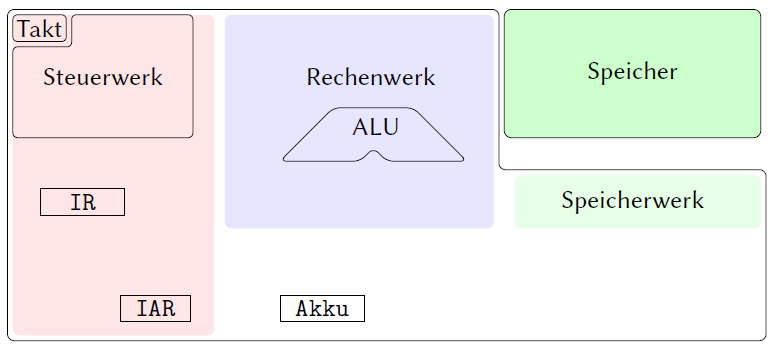
\includegraphics[width=\linewidth]{MIMA_simple.png}} \only<2|handout:2>{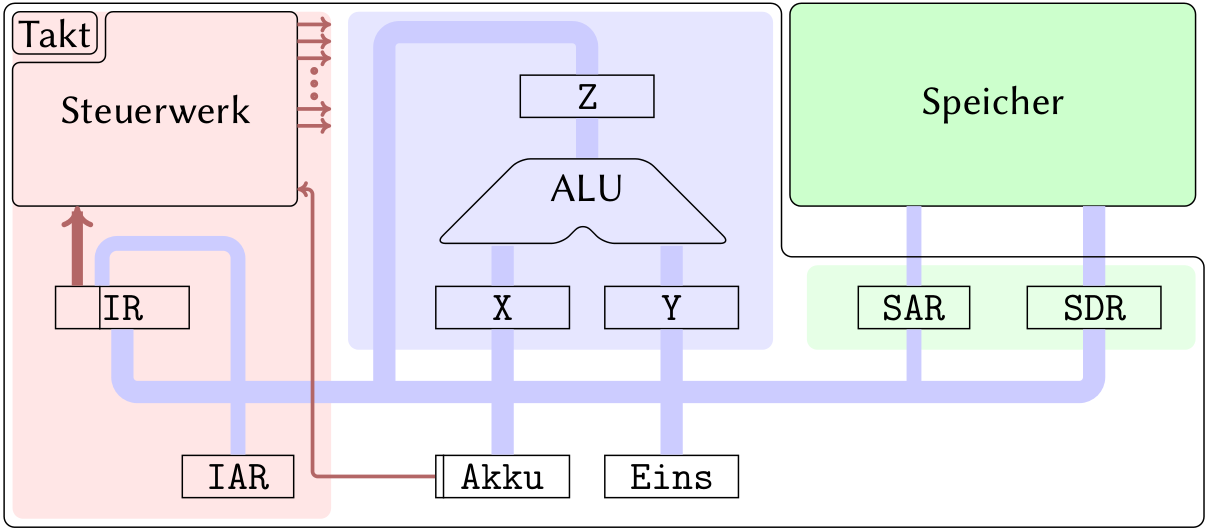
\includegraphics[width=\linewidth]{MIMA.png}}
\end{frame}

\begin{frame}{Minimalmaschine: Befehle}\small
\begin{columns}
	\begin{column}{0.6\textwidth}
		\begin{tabular}{|l|l|}
			\toprule
				% Zugriffsoperationen
				LDC $c$ & $c \rightarrow Akku$ \\
				LDV $a$ & $M(a) \rightarrow Akku$ \\
				STV $\alpha$ & $M(a) \leftarrow Akku$ \\
				LDIV $a$ & $M(M(a)) \rightarrow Akku$ \\
				STIV $a$ &$M(M(a)) \leftarrow Akku$ \\
				\midrule
				% Rechenoperationen
				ADD $a$ & $Akku + M(a) \rightarrow Akku$ \\
				AND $a$ & $Akku \ AND \ M(a) \rightarrow Akku$ \\
				OR $a$ & $Akku \ OR \ M(a) \rightarrow Akku$\\
				XOR $a$ & $Akku \ XOR \ M(a) \rightarrow Akku$\\
				NOT & Einskomplement von $Akku \rightarrow Akku$\\
				RAR & rotiert $Akku$ um 1 nach rechts $\rightarrow Akku$\\
				\midrule
				% Vergleichsoperationen
				EQL $a$ & $Akku \leftarrow \begin{cases}
											-1 & \text{, falls } Akku = M(a) \\
											0 & \text{, sonst} 
											\end{cases}$\\
				\midrule
				% Sprünge
				JMP $a$ & fahre fort mit Befehl an der Adresse $a$\\
				JMN $a$ & falls $Akku < 0$: JMP $a$\\
				HALT & stoppt die Mima\\
			\bottomrule	
		\end{tabular}
	\end{column}

	\begin{column}{0.32\textwidth}
		$c$: Konstante \\
		$a$: Adresse \\
		$M(a)$: Wert an Adresse $a$
	\end{column}
\end{columns}
\end{frame}

\begin{frame}{Minimalmaschine}
	\begin{exampleblock}{Eigenschaften}
		\begin{itemize}
		\item Adressen sind 20 Bit lang
		\item Werte sind 24 Bit lang
		\item Befehlscodierungen:
		\begin{itemize}
			\item 4 Bit für den OpCode und 20 Bit für einen Parameter (Adresse / Konstante)
			\item 8 Bit Befehl (Rest irrelevant)\\
			\includegraphics[width=100px]{MIMA_commands.png}\\
		\end{itemize} 
	\end{itemize}
	\end{exampleblock}
\end{frame}

\begin{frame}{Minimalmaschine}
	\begin{alertblock}{HALT}
		Jedes Programm muss mit HALT enden! Sonst läuft das Programm endlos weiter!
	\end{alertblock}

	\begin{alertblock}{Negative Konstanten}
		Negative Konstanten können nicht mit LDC geladen werden.\\
		Warum? \pause Unser Akku ist 24 Bit breit, aber wir können nur in die hinteren 20 Bit laden!
	\end{alertblock}
\end{frame}

\subsection{Aufgaben}
\begin{frame}{Minimalmaschine}
	\begin{exampleblock}{Aufgabe}
		Schreibe ein Programm, das eine an Adresse $a$ gegebene Zahl negiert und wieder in $a$ speichert.
	\end{exampleblock}
	\pause
	\begin{block}{Lösung}
			LDV $a$\\
			NOT\\
			STV $R$\\
			LDC 1\\
			ADD $R$\\
			STV $a$\\
			HALT
		\end{block}
\end{frame}

\begin{frame}{}
	\begin{exampleblock}{Aufgabe}
		An den Adressen $a$ und $b$ liegen zwei ganze Zahlen in Zweierkomplementdarstellung. Schreibe ein Programm, das $M(a)-M(b)$ errechnet und das Ergebnis an Adresse $c$ speichert.
	\end{exampleblock}

	% \begin{block}{Lösung}
	% 	% TODO
	% \end{block}
\end{frame}

\begin{frame}{Minimalmaschine}
	\begin{exampleblock}{Aufgabe}
		Sei $n \in \nN_+$. Schreibe ein Programm, das eine an Speicheradresse $a_1$ gegebene, positive, ganze Zahl Modulo $n$ errechnet und an Adresse $a_2$ ablegt.
	\end{exampleblock}
\end{frame}

\begin{frame}{Minimalmaschine}
	\begin{block}{Lösung: Modulo $n$}\small
		start: LDC $n$\\
		$\qquad$ NOT\\
		$\qquad$ STV $R$\\
		$\qquad$ LDC 1\\
		$\qquad$ ADD $R$\\
		$\qquad$ STV $NEGN$\\
		$\qquad$ LDV $a_1$ \\
		\medskip
		while:   ADD $NEGN$\\
		$\qquad$ JMN ende\\
		$\qquad$ JMP while\\
		\medskip
		ende:    STV $LOOPRESULT$\\
		$\qquad$ LDC $n$\\
		$\qquad$ ADD $LOOPRESULT$\\
		$\qquad$ STV $a_2$\\
		$\qquad$ HALT\\
	\end{block}
\end{frame}

\begin{frame}{}
	\begin{exampleblock}{Aufgabe}
		Wie kann man das für $n=2$ besser, d.h. mit weniger Anweisungen, machen?
	\end{exampleblock}
\pause
	\begin{block}{Lösung: Modulo 2}
		start:   LDC 1 //000000000000000000000001 \\
		$\qquad$ AND $a_1$ \\
		$\qquad$ STV $a_1$ \\
		$\qquad$ HALT
	\end{block}
\end{frame}


	% \begin{block}{Lösung}
	% 	% TODO
	% \end{block}

%%%%%%%%%% %%%%%%%%%%
\section{}
\questionframe
\lastframe
\mode<handout>{\slideThanks}
\end{document}